\documentclass[oneside, 12pt]{article}

\usepackage[slovene]{babel}    % slovenian language and hyphenation
\usepackage[utf8]{inputenc}    % make čšž work on input
\usepackage[T1]{fontenc}       % make čšž work on output
\usepackage[reqno]{amsmath}    % basic ams math environments and symbols
\usepackage{amssymb,amsthm}    % ams symbols and theorems
\usepackage{mathtools}         % extends ams with arrows and stuff
\usepackage{url}               % \url and \href for links
\usepackage{icomma}            % make comma a thousands separator with correct spacing
\usepackage{units}             % \unit[1]{m} and unitfrac
\usepackage{enumerate}         % enumerate style
\usepackage{array}             % mutirow
\usepackage[usenames]{color}   % colors with names
\usepackage{graphicx}          % images

\usepackage[bookmarks, colorlinks=true, linkcolor=black, anchorcolor=black,
  citecolor=black, filecolor=black, menucolor=black, runcolor=black,
  urlcolor=black, pdfencoding=unicode]{hyperref}  % clickable references, pdf toc
\usepackage[
  paper=a3paper,
  top=2cm,
  bottom=2cm,
  left=2cm,
  right=2cm,
%   textwidth=19cm,
% textheight=24cm,
]{geometry}  % page geomerty
\usepackage{pst-barcode}
\usepackage{auto-pst-pdf}

\newtheorem{izrek}{Izrek}
\newtheorem{posledica}{Posledica}

\theoremstyle{definition}
\newtheorem{definicija}{Definicija}
\newtheorem{opomba}{Opomba}
\newtheorem{zgled}{Zgled}

% basic sets
\newcommand{\R}{\ensuremath{\mathbb{R}}}
\newcommand{\N}{\ensuremath{\mathbb{N}}}
\newcommand{\Z}{\ensuremath{\mathbb{Z}}}
\renewcommand{\C}{\ensuremath{\mathbb{C}}}
\newcommand{\Q}{\ensuremath{\mathbb{Q}}}

% lists with less vertical space
\newenvironment{itemize*}{\vspace{-6pt}\begin{itemize}\setlength{\itemsep}{0pt}\setlength{\parskip}{2pt}}{\end{itemize}}
\newenvironment{enumerate*}{\vspace{-6pt}\begin{enumerate}\setlength{\itemsep}{0pt}\setlength{\parskip}{2pt}}{\end{enumerate}}
\newenvironment{description*}{\vspace{-6pt}\begin{description}\setlength{\itemsep}{0pt}\setlength{\parskip}{2pt}}{\end{description}}

\newcommand{\Title}{Kenguru}
\newcommand{\Author}{Jure Slak}
\title{\Title}
\author{\Author}
\date{\today}
\hypersetup{pdftitle={\Title}, pdfauthor={\Author}, pdfcreator={\Author},
            pdfproducer={\Author}, pdfsubject={}, pdfkeywords={}}  % setup pdf metadata

\pagestyle{empty}              % vse strani prazne
\setlength{\parindent}{0pt}    % zamik vsakega odstavka
\setlength{\parskip}{8pt}     % prazen prostor po odstavku
\setlength{\overfullrule}{30pt}  % oznaci predlogo vrstico z veliko črnine

\newcommand{\veliko}[1]{\scalebox{3}{\textbf{#1}}}
\newcommand{\srednje}[1]{\scalebox{2.4}{#1}}
\newcommand{\povezava}[1]{\begin{center}\vspace{-20pt}\Large \url{#1}\end{center}}

\begin{document}
\begin{flushleft}

\includegraphics[width=0.4\textwidth]{LogoDMFA_Mono.pdf}
\hfill
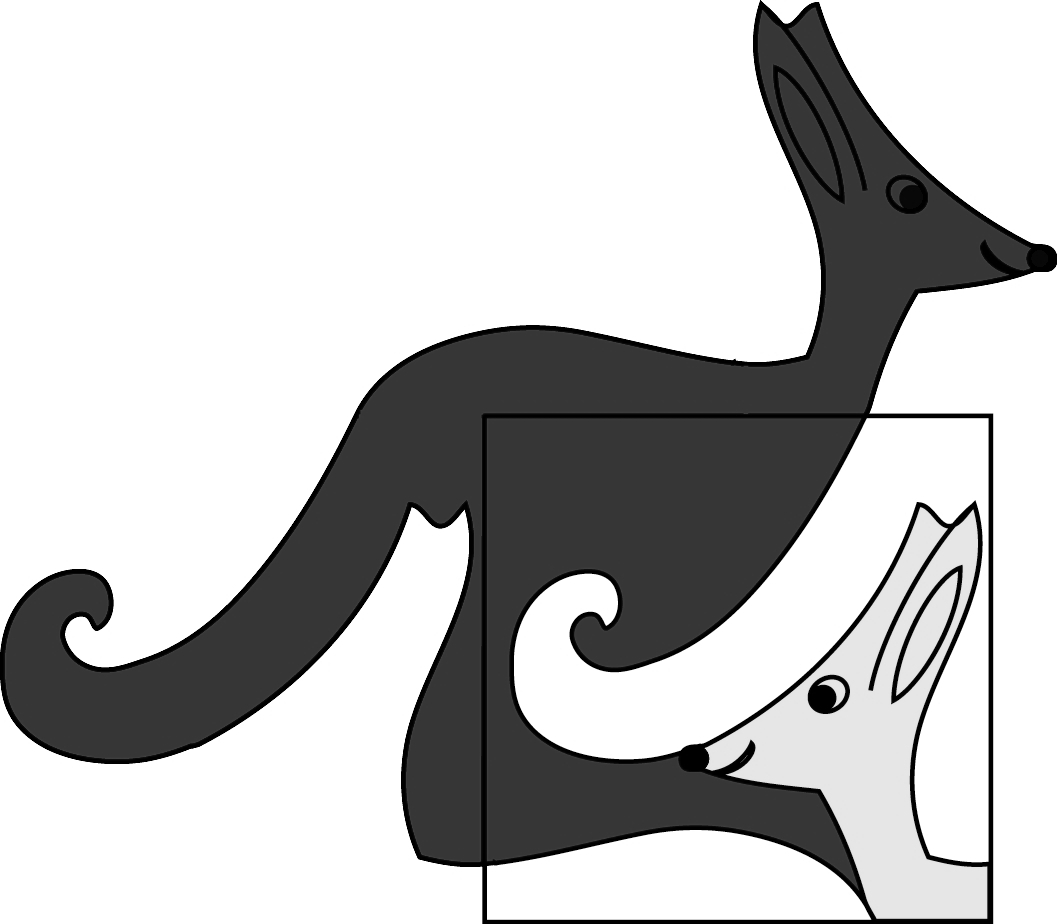
\includegraphics[width=0.4\textwidth]{logo_kangaroo.jpg}
\end{flushleft}

\setlength{\parskip}{40pt}
\fontsize{38}{40}\selectfont
DMFA Slovenije organizira tekmovanje študentov v znanju matematike.

Šolsko
tekmovanje bo v \textbf{četrtek, 17.\ 3.\ 2016, ob 17:00 na FMF}.

Najuspešnejši tekmovalci na šolskem delu tekmovanja prejmejo
bronasto priznanje, na državnem tekmovanju pa srebrno ali zlato priznanje.
Slednje lahko uveljavljate
tudi kot izjemni dosežek iz znanja za pridobitev Zoisove štipendije.

Prijavite se lahko z izpolnitvijo obrazca na \\
\texttt{www.dmfa.si/tekmovanja/MaVS/Prijava.aspx} \\
do 16.\ 3.\ 2016 do 12:00.
\begin{center}
\scalebox{2}{
\begin{pspicture}(2in,2in)
  \psbarcode{http://www.fmf.uni-lj.si/si/obvestila/36865/}{eclevel=M}{qrcode}
\end{pspicture}}
\end{center}



\end{document}
% vim: syntax=tex
% vim: spell spelllang=sl
% vim: foldlevel=99
% Latex template: Jure Slak, jure.slak@gmail.com

